\documentclass[presentation,english,usenames,dvipsnames]{beamer}
\usepackage[utf8]{inputenc}
\usepackage{babel}
\usepackage{graphicx}
\usepackage{longtable}
\usepackage{float}
\usepackage{wrapfig}
\usepackage{soul}
\usepackage{textcomp}
\usepackage{marvosym}
\usepackage{wasysym}
\usepackage{latexsym}
\usepackage{amssymb}
\usepackage{hyperref}
\tolerance=1000
\usepackage{listings}
\usepackage[iso]{isodate}
\usepackage[font=scriptsize, skip=0pt]{caption}
\usepackage[font=scriptsize, skip=0pt]{subcaption}
\usepackage{pgfplots, pgfplotstable}
\pgfplotsset{compat=1.14}
\usepackage{tikz}
\usetikzlibrary{fit, shapes}
\pgfdeclarelayer{background}
\pgfsetlayers{main,background}

\title[Peer-to-Peer Incentives]{Incentivizing Peers to contribute in a
Low-Latency Name-Lookup Service}
\author{Marc Lehmann}
\subtitle{Final Master Talk}
\date{\today}


\usetheme{Comsys}
% Adjust the title font size, because my title spans 3 lines otherwise.
\setbeamerfont{title}{size*={16}{26.4},series=\bfseries}

\begin{document}

\setbeamertemplate{footline}[empty]
\begin{frame}
  \titlepage
\end{frame}

\setbeamertemplate{footline}[comsys]

\begin{frame}{Motivation}
  \begin{itemize}
    \item Name-mapping service important to facilitate communication
    \begin{itemize}
      \item names to IPs (DNS)
      \item people to devices (instant messaging)
    \end{itemize}
    \item Privacy concerns in centralized systems
    \begin{itemize}
      \item Server gets a lot of information about whom a user communicates with
      \item Can build user profiles
      \item Can become target for others who want to build profiles
    \end{itemize}
    \item Spread requests to many different nodes in a DHT
    \item Requires lots of nodes\rightarrow users need to participate
          themselves
  \end{itemize}
\end{frame}

\begin{frame}{Encouraging peers to contribute}
  \begin{itemize}
    \item Assume peers are selfish
    \item Only leverage: users want good service
    \item Give bad peers bad service (delayed responses)
    \item Track how good peers are via a reputation system
    \item Existing solutions to track reputation insufficient
    \begin{itemize}
      \item Assume a central authority {\color{gray}\tiny[Gupta et al.]}
      \item Aren't Scalable {\color{gray}\tiny[Zhou et al.]}
      \item Or propose using another DHT {\color{gray}\tiny[Feldman et al.]},
            introducing additional latency
    \end{itemize}
    \item Solution: Create small subsets of peers (query groups),
          broadcast/gossip reputation updates in those
  \end{itemize}
\end{frame}

\begin{frame}{Query Groups (Chord)}
  \begin{minipage}{0.5\textwidth}
    \begin{itemize}
      \item Using Chord to illustrate
      \item Need to be able to reach peers in finger table
      \item Need to share a query group with each of these peers
      \item (Not necessarily the same for all)
    \end{itemize}
  \end{minipage}% This comment is necessary to remove any space between the minipages
  \begin{minipage}{0.5\textwidth}
    \begin{figure}
      \centering
      \begin{tikzpicture}
        \begin{scope}[every node/.style={
          circle,
          fill=black,
          inner sep=0pt,
          minimum size=5pt
          }]
          \node[minimum size=8pt] (A) at (90:2) {};
          \node[red] (B) at (30:2) {};
          \node[blue] (C) at (330:2) {};
          \node[violet] (D) at (270:2) {};
          \node[OliveGreen] (E) at (210:2) {};
          \node (F) at (150:2) {};
        \end{scope}

        \draw (B) -- (C)[draw=none] node[midway, sloped] {\ldots};
        \draw (C) -- (D)[draw=none] node[midway, sloped] {\ldots};
        \draw (D) -- (E)[draw=none] node[midway, sloped] {\ldots};
        \draw (E) -- (F)[draw=none] node[midway, sloped] {\ldots};
        \draw (F) -- (A)[draw=none] node[midway, sloped] {\ldots};

        \draw[->] (A) -- (B);
        \draw[->] (A) -- (C);
        \draw[->] (A) -- (D);
        \draw[->] (A) -- (E);

        \begin{pgfonlayer}{background}
          \begin{scope}[every node/.style={
            ellipse,
            draw=black,
            thick,
            inner sep=0pt,
            inner xsep=0pt,
            inner ysep=0pt,
            opacity=0.5
          }]
            \invisible{
              \node[fit=(A)(B), fill=red!30, rotate=-30] {};
            }
            \invisible{
              \node[fit=(A)(C)(D), fill=violet!30, rotate=18, xshift=-15pt] {};
            }
            \invisible{
              \node[fit=(A)(E), fill=OliveGreen!30, rotate=-30,
                    inner xsep=-15pt] {};
            }
          \end{scope}
        \end{pgfonlayer}
      \end{tikzpicture}
    \end{figure}
  \end{minipage}
\end{frame}

\begin{frame}{Query Groups (Chord)}
  \begin{minipage}{0.5\textwidth}
    \begin{itemize}
      \item \visible<1->{Join query group with red peer}
      \item \visible<2->{Join query group with blue peer}
      \item \visible<2->{Purple peer is also in that group}
      \item \visible<3->{Join query group with green peer}
    \end{itemize}
  \end{minipage}% This comment is necessary to remove any space between the minipages
  \begin{minipage}{0.5\textwidth}
    \begin{figure}
      \centering
      \begin{tikzpicture}
        \begin{scope}[every node/.style={
          circle,
          fill=black,
          inner sep=0pt,
          minimum size=5pt
          }]
          \node[minimum size=8pt] (A) at (90:2) {};
          \node[red] (B) at (30:2) {};
          \node[blue] (C) at (330:2) {};
          \node[violet] (D) at (270:2) {};
          \node[OliveGreen] (E) at (210:2) {};
          \node (F) at (150:2) {};
        \end{scope}

        \draw (B) -- (C)[draw=none] node[midway, sloped] {\ldots};
        \draw (C) -- (D)[draw=none] node[midway, sloped] {\ldots};
        \draw (D) -- (E)[draw=none] node[midway, sloped] {\ldots};
        \draw (E) -- (F)[draw=none] node[midway, sloped] {\ldots};
        \draw (F) -- (A)[draw=none] node[midway, sloped] {\ldots};

        \draw[->] (A) -- (B);
        \draw[->] (A) -- (C);
        \draw[->] (A) -- (D);
        \draw[->] (A) -- (E);

        \begin{pgfonlayer}{background}
          \begin{scope}[every node/.style={
            ellipse,
            draw=black,
            thick,
            inner sep=0pt,
            inner xsep=0pt,
            inner ysep=0pt,
            opacity=0.5
          }]
            \visible<1->{
              \node[fit=(A)(B), fill=red!30, rotate=-30] {};
            }
            \visible<2->{
              \node[fit=(A)(C)(D), fill=violet!30, rotate=18, xshift=-15pt] {};
            }
            \visible<3->{
              \node[fit=(A)(E), fill=OliveGreen!30, rotate=-30,
                    inner xsep=-15pt] {};
            }
          \end{scope}
        \end{pgfonlayer}
      \end{tikzpicture}
    \end{figure}
  \end{minipage}
\end{frame}

\begin{frame}{Query Groups (Chord)}
  \begin{minipage}{0.5\textwidth}
    \begin{itemize}
      \item Query groups also contain other peers
      \item Everybody knows everybody's reputation
    \end{itemize}
  \end{minipage}% This comment is necessary to remove any space between the minipages
  \begin{minipage}{0.5\textwidth}
    \begin{figure}
      \centering
      \begin{tikzpicture}
        \begin{scope}[every node/.style={
          circle,
          fill=black,
          inner sep=0pt,
          minimum size=5pt
          }]
          \node[minimum size=8pt] (A) at (90:2) {};
          \invisible{\node[red] (B) at (30:2) {};}
          \node[blue] (C) at (330:2) {};
          \node[violet] (D) at (270:2) {};
          \invisible{\node[OliveGreen] (E) at (210:2) {};}
          \invisible{\node (F) at (150:2) {};}
        \end{scope}
        \begin{scope}[every node/.style={
          circle,
          draw=black,
          inner sep=0pt,
          minimum size=5pt
          }]
          \node (G) at (90:1) {};
          \node (H) at (180:0.5) {};
          \node (I) at (135:1.2) {};
          \node (J) at (280:1.3) {};
          \node (K) at (0:1) {};
          \node (L) at (330:1) {};
        \end{scope}

        \draw (A) -- (C)[draw=gray, opacity=0.8];
        \draw (A) -- (D)[draw=gray, opacity=0.8];
        \draw (A) -- (G)[draw=gray, opacity=0.8];
        \draw (A) -- (H)[draw=gray, opacity=0.8];
        \draw (A) -- (I)[draw=gray, opacity=0.8];
        \draw (A) -- (J)[draw=gray, opacity=0.8];
        \draw (A) -- (K)[draw=gray, opacity=0.8];
        \draw (A) -- (L)[draw=gray, opacity=0.8];
        \draw (C) -- (D)[draw=gray, opacity=0.8];
        \draw (C) -- (G)[draw=gray, opacity=0.8];
        \draw (C) -- (H)[draw=gray, opacity=0.8];
        \draw (C) -- (I)[draw=gray, opacity=0.8];
        \draw (C) -- (J)[draw=gray, opacity=0.8];
        \draw (C) -- (K)[draw=gray, opacity=0.8];
        \draw (C) -- (L)[draw=gray, opacity=0.8];
        \draw (D) -- (G)[draw=gray, opacity=0.8];
        \draw (D) -- (H)[draw=gray, opacity=0.8];
        \draw (D) -- (I)[draw=gray, opacity=0.8];
        \draw (D) -- (J)[draw=gray, opacity=0.8];
        \draw (D) -- (K)[draw=gray, opacity=0.8];
        \draw (D) -- (L)[draw=gray, opacity=0.8];
        \draw (G) -- (H)[draw=gray, opacity=0.8];
        \draw (G) -- (I)[draw=gray, opacity=0.8];
        \draw (G) -- (J)[draw=gray, opacity=0.8];
        \draw (G) -- (K)[draw=gray, opacity=0.8];
        \draw (G) -- (L)[draw=gray, opacity=0.8];
        \draw (H) -- (I)[draw=gray, opacity=0.8];
        \draw (H) -- (J)[draw=gray, opacity=0.8];
        \draw (H) -- (K)[draw=gray, opacity=0.8];
        \draw (H) -- (L)[draw=gray, opacity=0.8];
        \draw (I) -- (J)[draw=gray, opacity=0.8];
        \draw (I) -- (K)[draw=gray, opacity=0.8];
        \draw (I) -- (L)[draw=gray, opacity=0.8];
        \draw (J) -- (K)[draw=gray, opacity=0.8];
        \draw (J) -- (L)[draw=gray, opacity=0.8];
        \draw (K) -- (L)[draw=gray, opacity=0.8];

        \invisible{\draw (B) -- (C)[draw=none] node[midway, sloped] {\ldots};}
        \invisible{\draw (C) -- (D)[draw=none] node[midway, sloped] {\ldots};}
        \invisible{\draw (D) -- (E)[draw=none] node[midway, sloped] {\ldots};}
        \invisible{\draw (E) -- (F)[draw=none] node[midway, sloped] {\ldots};}
        \invisible{\draw (F) -- (A)[draw=none] node[midway, sloped] {\ldots};}

        \invisible{\draw[->] (A) -- (B);}
        \invisible{\draw[->] (A) -- (C);}
        \invisible{\draw[->] (A) -- (D);}
        \invisible{\draw[->] (A) -- (E);}

        \begin{pgfonlayer}{background}
          \begin{scope}[every node/.style={
            ellipse,
            draw=black,
            thick,
            inner sep=0pt,
            inner xsep=0pt,
            inner ysep=0pt,
            opacity=0.5
          }]
            \invisible{
              \node[fit=(A)(B), fill=red!30, rotate=-30] {};
            }
            \node[fit=(A)(C)(D), fill=violet!30, rotate=18, xshift=-15pt] {};
            \invisible{
              \node[fit=(A)(E), fill=OliveGreen!30, rotate=-30,
                    inner xsep=-15pt] {};
            }
          \end{scope}
        \end{pgfonlayer}
      \end{tikzpicture}
    \end{figure}
  \end{minipage}
\end{frame}

\begin{frame}
\end{frame}

\begin{frame}{Query Groups (Kademlia/P-Grid)}
  \begin{itemize}
    \item View keys as bitstring
    \item Peers have a routing prefix (bitstring): store keys that start with
          that prefix
    \item Peers are in contact with others with the same routing prefix
          (replication)
    \item Other routing prefixes: know other peers closer to them
  \end{itemize}
  \begin{figure}
    \centering
    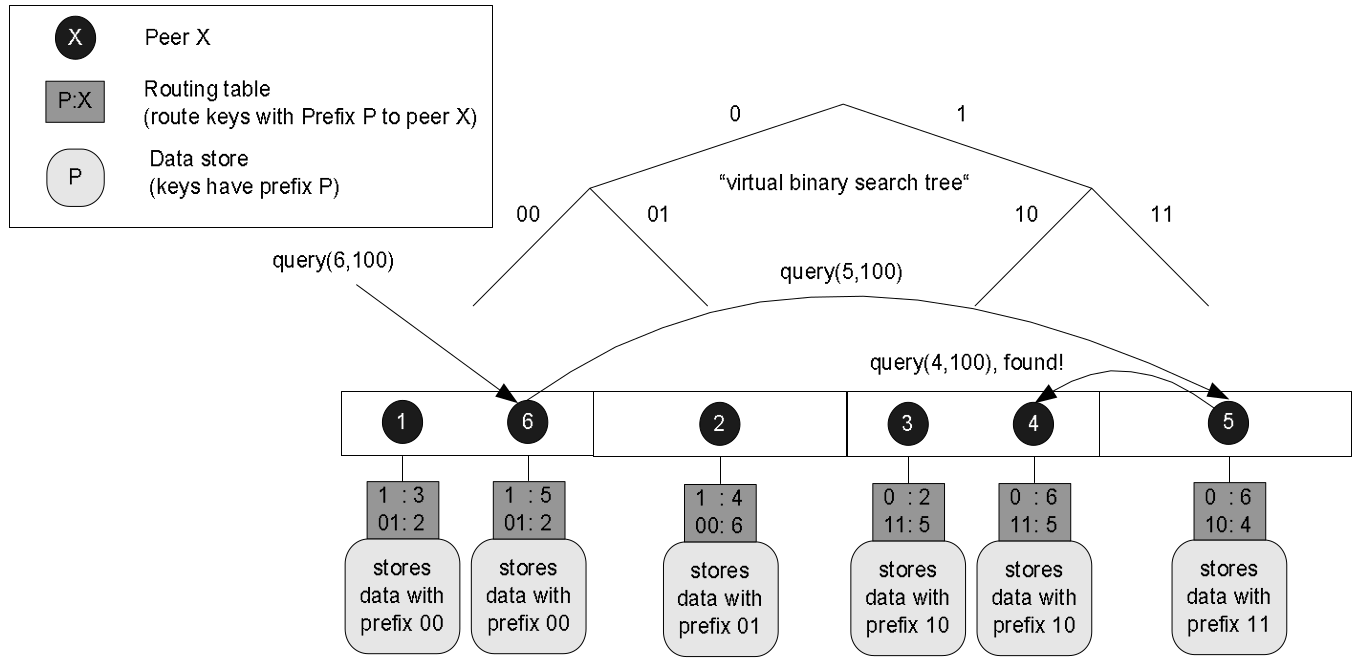
\includegraphics[width=0.5\textwidth]{p-grid}
    \caption*{\tiny From \emph{P-Grid: A Self-organizing Structured P2P System}}
  \end{figure}
\end{frame}

\begin{frame}{Query Groups (Kademlia/P-Grid)}
  \begin{itemize}
    \item Dashed: Same routing prefix, replication (sync groups)
    \item Solid: Query groups
  \end{itemize}
  \begin{figure}
    \centering
    \begin{tikzpicture}
      \begin{scope}[every node/.style={draw}]
        \node[color=red] (A) at (0:2) {P: 001};
        \node[color=blue] (B) at (45:2) {P: 001};
        \node[color=red] (C) at (90:2) {P: 001};
        \node[color=blue] (D) at (135:2) {P: 010};
        \node[color=OliveGreen] (E) at (180:2) {P: 010};
        \node[color=blue] (F) at (225:2) {P: 101};
        \node[color=red] (G) at (270:2) {P: 101};
        \node[color=OliveGreen] (H) at (315:2) {P: 101};
      \end{scope}

      \path (A) edge[thick,dashed,bend right=15] (B);
      \path (B) edge[thick,dashed,bend right=15] (C);
      \path (A) edge[thick,dashed,bend left=15] (C);
      \path (D) edge[thick,dashed,bend right=15] (E);
      \path (F) edge[thick,dashed,bend right=15] (G);
      \path (G) edge[thick,dashed,bend right=15] (H);
      \path (F) edge[thick,dashed,bend left=15] (H);
      \path (A) edge[thick,color=red,bend left=20] (C);
      \path (C) edge[thick,color=red] (G);
      \path (A) edge[thick,color=red,bend right=15] (G);
      \path (B) edge[thick,color=blue] (D);
      \path (D) edge[thick,color=blue,bend left=15] (F);
      \path (B) edge[thick,color=blue] (F);
      \path (E) edge[thick,color=OliveGreen] (H);
    \end{tikzpicture}
  \end{figure}
\end{frame}

\begin{frame}{Why do we need incentives?}
  \begin{itemize}
    \item Maybe we don't
    \item "Just distribute software that contributes to the DHT, people will be
          too lazy to change it for a small benefit"
          \begin{itemize}
            \item Some alternative implementation may opt to leave it out
            \item Maybe for performance, maybe for security
          \end{itemize}
    \item Assume the worst case, be ready for reality
    \item Just nice to know if it would work
  \end{itemize}
\end{frame}

\end{document}
